
	\chapter{CoAP}\label{ch:coap}
	In this chapter we analyze the Constrained Application Protocol (CoAP) and its main features, in order to make the reading more comfortable,
	we will skip some technical details that are not crucial to the understanding of basic concept of the protocol.\newline
	In case you find yourself interested by CoAP and you want to examine all the details you can consult
	the RFC 7252 defined by IETF ~\cite{rfccoap}. \newline
	We will analyze the request/response model followed by its semantics to proceed with the detailed description of CoAP messages, in order to understand how the protocol tries to limit the overhead as much as possible; then we will analyze how transmission occurs.\newline
	Then we will focus on secondary aspects of the protocol: caching, proxying and discovery.\newline
	To conclude we will discuss the security of CoAP and have a little comparison with its direct competitor MQTT, in the end we will have an overview of the available implementations of the protocol.\newline
	
	CoAP stands for Constrained Application Protocol, it is specialized to work with constrained nodes and networks where computational power is low and power consumption is not negligible.\newline
	In this context, nodes are characterized from small amount of memory and by dated micro-controller.\newline

	CoAP belongs to the UDP based protocol family; UDP has been chosen for performance reason, due to the fact that a constrained devices may not be powerful enough to handle a protocol like HTTP that relies on TCP.\newline
	
	CoAP can be seen as a lightweight version of HTTP that meet with the technical specification of sensor and embedded machine; as we will see in detail in the following chapter, CoAP and HTTP share some technical details, because CoAP is designed to easily translate to HTTP in order to achieve a simplified integration with the web.\newline

	In order to be a lightweight protocol, CoAP treats data in a very careful way in order to avoid heavy communications, that is why each message has a short fixed length binary header of four byte only. Even if CoAP is light, it has a reliability mechanism that allows the sender to know if the message sent has been received, of course it is not comparable to the one specified by TCP, in fact TCP provides us message in order while COAP does not.
	TCP has checksum to check whether a message is corrupted or not, CoAP lacks this integrity check .\newline
	
	CoAP specifies two types of messages:
	\begin{itemize}
		\item Confirmable (CON)
		\item Non-Confirmable (NON)
	\end{itemize}
	Only CON messages are considered reliable, in fact a confirmable message is retransmitted using a default timeout plus an exponential back-off between retransmission, until the recipient does not send an ACK message back to the sender.\newline
	As CoAP is built upon UDP, it allows multicast IP destination addresses, thus this protocol can handle multicast requests.\newline
	
	\section{Request/Response model}
	CoAP request and response semantics are carried in messages with the aid of method and response code; optional information, such as URI and payload are carried as options.\newline
	Token and Message ID are separate concept but at a first look they seem the same: the token matches a response
	with a request while the Message ID is used to detect duplicates and for optional reliability.\newline
	
	A message regardless of being a CON or NON carries a request; when the server receives the request, it sends back an ACK message that could have the response or not. In the latter case the server will
	send a new message with the response, this is done to stop the retransmission of a certain request by the client.\newline
	The first case is known as piggybacked response, the second as separate response. Whenever possible the server will prefer the piggybacked way, of course. However if the request requires some times to be processed, the protocol will rely on the separate response.\newline
	If the request is sent as a NON message, then the response is a new NON message, but the server may send a CON message.\newline
	
	In order to be as fast as possible in fulfilling requests, CoAP supports caching to provide piggybacked responses.\newline
	
	Figure \ref{fig:coap0} illustrates two simple client/server communications.
	
	\begin{figure}
		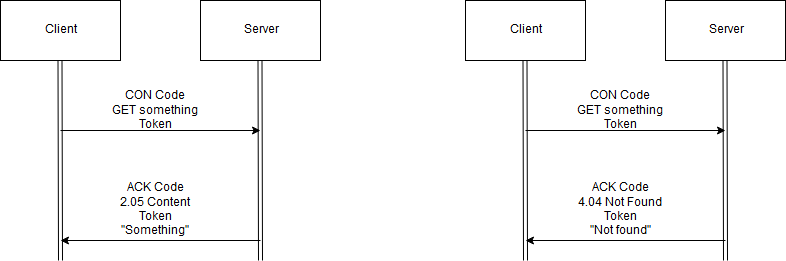
\includegraphics[width=\linewidth]{coap-img0.png}
		\caption{Example of CoAP request/response model, at left the request is fulfilled, on the right it is not.}
		\label{fig:coap0}
	\end{figure}
	
	CoAP uses \emph{methods} in a similar way to HTTP, the supported methods are: \newline
	\begin{itemize}
		\item GET
		\item PUT
		\item POST
		\item DELETE
	\end{itemize}
	But new methods could be added in future revision of the protocol.\newline
	
	\section{Semantics}
	
	CoAP works in a similar way to HTTP, the client sends one or more requests to the server, which sends back responses.\newline
	The main difference between CoAP and HTTP is the lack of a previously established connection because CoAP messages are exchanged asynchronously.\newline
	A CoAP request is made up by a method, the resource which the method will be applied,
	a payload and an Internet media type and optional metadata.\newline
	Each method in a request has its own semantics:
	\begin{itemize}
		\item A GET request retrieves a resource specified by the request URI.
		It is considered secure because it only needs to retrieve the resource.
		
		\item When the server receives a POST request it processes the resource enclosed in the request.
		What is performed is determined by the origin server and not by the protocol.
		If a resource has been created on the server, the response should be a 2.01 and should include the URI of the new resource.
		If a new resource is not created by a POST request, the server should send back a 2.04 response.
		
		\item A PUT request creates or updates the resource specified by the request URI.
		If the resource exists, then it is updated and the server should send back a 2.04 response.
		On the other hand if the resource did not exist, the server creates it and sends back a 2.01 response.
		
		\item When the server receives a DELETE request it should delete the specified resource.
		
	\end{itemize}
	
	A CON or NON message with the Code field set with all the information needed is a request.\newline
	When the server receives a request, it is interpreted and the server sends back a CoAP response that has the same token generated by the client.\newline
	A response is a CoAP message that has the Code field set to a Response Code.\newline

	The available response codes are listed in table \ref{tab:table13}

		\begin{table}[h!]
		\begin{center}
			\begin{tabular}{|c|c|c|}
				\hline
				\textbf{2.xx Success} & \textbf{4.xx Client Error} & \textbf{5.xx Server Error}\\\hline
				2.01 Created & 4.00 Bad Request & 5.00 Internal Server Error\\\hline
				2.02 Deleted & 4.01 Unauthorized & 5.01 Not Implemented\\\hline
				2.03 Valid & 4.02 Bad Option & 5.02 Bad Gateway\\\hline
				2.04 Changed & 4.03 Forbidden & 5.03 Service Unavailable\\\hline
				2.05 Content & 4.04 Not Found & 5.04 Gateway Timemout\\\hline
				- & 4.05 Method Not Allowed & 5.05 Proxying Not Supported\\\hline
				- & 4.06 Not Acceptable & -\\\hline
				- & 4.12 Precondition Failed & -\\\hline
				- & 4.13 Request Entity Too Large & -\\\hline
				- & 4.15 Unsupported Content-Format & -\\
   				\hline
			\end{tabular}
			\caption{CoAP methods.}
			\label{tab:table13}
		\end{center}
	\end{table}
	
	In general, if the response code belongs to the 2.xx class then it means the server received, understood and processed the request correctly, otherwise if the response belongs to the 4.xx class then the request contained errors and the server refused to process it. On the other hand if the response belongs to the 5.xx class then the request was correct but the server was unable to fulfill it.\newline
	The semantics of each response is available in the RFC.\newline
	
	The response is returned in the ACK regardless it is a success or a failure; there is no need to send a separate message.\newline
	The server is free to send a piggybacked response or a separate response, and the client must be prepared to receive both.\newline
	A separate response is used when the server might need some time to acquire a resource and perform the client request; for this reason, one possible implementation is the following:
	\begin{itemize}
		\item When the server receives a request, it immediately sends back an Empty ACK.
		\item Then the server will try to obtain the specified resource.
		\item When the resource has been obtained and the request performed, the server sends back the response.
		It sends the response as a CON message and waits the Empty ACK message from the client.
	\end{itemize}
	If the server receives the same message multiple times, and it has just sent an ACK message, it must not send back the response in another ACK.\newline
	
	When the request is a NON message, the response should be returned in a NON message as well.\newline
	An important thing to keep in mind is that a client must be prepared to receive a NON response even if the request was a CON message, or vice-versa a CON response in reply to a NON request.\newline
	
	A response matches a request if they have the same token and they match additional information like the address.\newline
	The token is used to identify concurrent requests from the same client; the client should generate tokens that are unique for a given source/destination endpoint pair.\newline
	If TLS is not used, a client should generate nontrivial, randomized token to avoid trivial spoofing of responses.\newline
	
	The rules for matching a response to a request are the following:
	\begin{itemize}
		\item The source of the response must match with the destination of the original request.
		\item In a piggybacked response, the Message ID of the CON request and the ACK must match; even the token of the CON message must match with token of the ACK message.
	\end{itemize}
	A request may carry some options; CoAP defines a set of options that are used in requests and even in responses,
	the list of options is available in the RFC.
	
	A payload may be included in both requests and responses, but only if the method or the Response Code allows it; if a recipient receives a request and the payload is not expected, the recipient must ignore it.
	
	When a request is fulfilled, then the response includes a payload which is a representation of a resource in a specific format, this format is specified by the \emph{Internet Media Type} in the \emph{Content-Format Option}.\newline
	If the Content-Format Option is missing, it should be inferred; the inclusion of the \emph{Content-Format Option} in a response is strongly recommended.\newline
	
	If a response, which specifies a certain client or server error is returned, without the Content-Format, then the payload is a diagnostic payload that contains a human-readable message encoded in UTF-8 in the Net-Unicode form.\newline
	
	A server could provide a resource in multiple ways, in order to specify the preferred format the client must add it in the Accept Option, and if the server can satisfy the request it will return a response with the appropriate payload format.\newline
	
	\section{Message Structure}
	Figure \ref{fig:coapheader} illustrates the CoAP header.\\
	\begin{figure}[h]
		\begin{bytefield}[bitwidth=1.1em]{32}
			\bitheader{0-31} \\
			\begin{rightwordgroup}{CoAP Header}
				\bitbox{2}{Ver}
				& \bitbox{2}{T}
				& \bitbox{4}{TLK}
				& \bitbox{8}{Code}
				& \bitbox{16}{Message Id}
			\end{rightwordgroup}
			\\\bitbox{32}{Token (if any, token of TKL bytes)}\\
			& \bitbox{32}{Options (if any)}\\
			& \bitbox{32}{Payload (if any)}
		\end{bytefield}
		\label{fig:coapheader}
		
	\end{figure}
	
	A CoAP message is encoded in a binary format and consist of:\newline
	\begin{itemize}
		\item A header
		\item A variable length token
		\item Zero or more options
		\item An optional payload
	\end{itemize}
	The header is 4 byte long, the token has a variable length, which can be between 0 and 8 bytes, the options and payload sizes are variable.\newline
	The header consist of five parameters:\newline
	\begin{enumerate}
		\item \texttt{Ver}: specify the CoAP version number with 2 bits, a CoAP implementation must set this field to 1, other values are reserved for future version, a message with unknown version number must be ignored.
		\item \texttt{T}: specifies the message's type with 2 bits:
		\begin{enumerate}
			\item 00 CON message
			\item 01 NON message
			\item 10 ACK message
			\item 11 RST message
		\end{enumerate}
		\item \texttt{TKL}: specifies the token length with 4 bits, lengths from nine to fifteen are reserved and must not be used and must be treated like a message error format.
		\item \texttt{Code}: this field is 8 bit long, the first 3 most significant bits specify the class, and the 5 least significant bits specify the details.
		The message code is specified in this way: “c.dd” where c is the class and dd the details.
		\item \texttt{Message ID}: it is used to identify a message, it is also used to detect duplicates and to match ACK/RST, its dimension is 16 bit.
	\end{enumerate}
	
	The token value is used to link requests and responses.\newline

	Then there are zero or more options; an option can be followed by: the end of the message, another option or by the payload.\newline
	Each option instance specifies an Option number, its length and the value itself.\newline
	Each instance must appear in order of its option number because delta encoding is used between them in order to keep the option fields as short as possible.\newline
	
	The structure is the following:\newline
	\begin{itemize}
		\item \texttt{Option delta}: specifies a value between 0 and 12 and is used as the difference between the Option Number of the current option instance and the previous one, its length is 4 bits.
		Values between 13 and 15 are reserved.
		If the value is 15 the message must be treated as message format error.
		\item \texttt{Option length}: specifies a value between 0 and 12 and indicates the length of the Option value.
		Its length is 4 bits and values between 13 and 15 are reserved, as before 15 must be treated as message format error.
		\item \texttt{Value}: a sequence of exactly Option Length bytes.
	\end{itemize}

	At the end, if present and of non-zero length, there is the payload prefixed by a payload marker of one byte: \texttt{0xFF}.\newline
	The payload length is not specified but calculated from the datagram size; on the other hand if the payload marker is absent the payload length is zero.\newline
	If the payload marker is present but followed by a zero-length payload, then the message must be treated like a message error format.\newline
	A CoAP message is transferred via one the following protocol: UDP, DTLS, SMS, TCP, and SCTP while UDP-lite and UDP zero checksum are not supported.\newline

	
	\section{Message transmission}
	The communication between endpoints is asynchronous, so take in mind that messages may arrive out of order, appear duplicated or go missing due to the unreliability of UDP.\newline
	As said, CoAP define a reliability mechanism, but the usage of CON message is not mandatory. This mechanism is different from the TCP reliability model and its features are the following:\newline
	\begin{itemize}
		\item Stop and wait retransmission reliability with exponential back-off, only for CON messages.
		\item Duplicate detection for both CON and NON messages.
	\end{itemize}

	A chosen endpoint is the source or the destination of a message and it is identified by the security mode; we will talk about it later, but if there is no active security mode, the endpoint is identified by an IP address and a UDP port number.\newline
	When a message is transmitted in a reliable way, it is marked as CON in the header and it always carries either a request or response, unless it is used only to elicit a RST message, in which case it is Empty.\newline
	There are two possible scenarios when the recipient receives a message:\newline
		\begin{itemize}
		\item It can acknowledge the message by sending an ACK with the same Message ID; the message must carry a response or be empty.
		\item Otherwise if the recipient is not capable of handling the message, it must: reject the message by sending a RST that matches the Message ID of the CON message and it must be empty, or ignore it.
	\end{itemize}

	To reject an ACK or RST message, an endpoint can simply ignore the message, on the other hand
	the recipient of an ACK or RST must not respond with an ACK or RST.\newline
	
	The sender retransmits the CON message at exponentially increasing intervals, 
	until it receives an ACK or stop because it runs out of attempts.\newline
	The retransmission is governed by a timeout and by an attempts counter.\newline
	When a new CON is transmitted, the initial timeout is set to a random duration between
	\texttt{ACK\_TIMEOUT} 
	and \texttt{ACK\_TIMEOUT$\cdot$ACK\_RANDOM\_FACTOR}, while the retransmission counter is set to 0.\newline
	\texttt{ACK\_TIMEOUT} and \texttt{ACK\_RANDOM\_FACTOR} are constants defined by the final implementation of the protocol.\newline
	Every time the timeout triggers and the counter is less than \texttt{MAX\_RETRANSMIT}, the message is retransmitted, the counter is incremented and the timeout is doubled.\newline
	If the retransmission counter is greater than \texttt{MAX\_RETRANSMIT} or the sender receives a RST message, then the retransmission is aborted.\newline
	Of course, if the sender receives an ACK the transmission is considered successful.\newline
	An endpoint may also give up in attempting to obtain an ACK even before reaching the \texttt{MAX\_RETRANSMIT} counter; for instance, the application may cancel the request because it is no more interested in the response.\newline
	
	When a message is transmitted without reliability the recipient must not send back an ACK message.\newline
	If the recipient is not capable of handling a message because it lacks content to process or because it is malformed, the message must be rejected.\newline
	
	A recipient might receive a NON message multiple times within \texttt{NON\_LIFETIME}.\newline
	The recipient should process the request only once; every duplicate message should be ignored.\newline
	The message size must be kept small enough to fit into the link layer packet; of course this is not always possible.\newline
	CoAP defines an upper bound to the message size, as a general rule a CoAP message should fit within a single IP packet end up bringing undesirable packet fragmentation.\newline
	The maximum transmission unit (MTU) is 1280 byte if no other optimal values is known.\newline
	As you may have noticed we have cited some variables without specifying their values, the default values are shown in \ref{tab:table3}.\newline
	
		\begin{table}[h!]
		\begin{center}
			\begin{tabular}{|l|l|}
				\hline
				\textbf{Name} & \textbf{Default value}\\\hline
					\texttt{ACK\_TIMEOUT} &	2 seconds\\\hline
					\texttt{ACK\_RANDOM\_FACTOR} & 1.5 \\\hline
					\texttt{MAX\_RETRANSMIT} & 4 \\\hline
					\texttt{NSTART} & 1 \\\hline
					\texttt{DEFAULT\_LEISURE} &	5 seconds \\\hline
					\texttt{PROBING\_RATE} & 1 byte/second \\\hline
			\end{tabular}
			\caption{List of constants defined by CoAP.}
			\label{tab:table3}
		\end{center}
	\end{table}

	The values listed in table \ref{tab:table3} are recommended in order to avoid congestion on the Internet, of course an implementation can customize these values in order to meet some special environment requirements.\newline
	Considering that \texttt{ACK\_TIMEOUT}, \texttt{ACK\_RANDOM\_FACTOR} and \texttt{MAX\_RETRANSMIT} influence the time of retransmission, thus they also influence how long certain information needs to be kept in memory by an implementation.\newline
	
	\section{Caching}
	In order to speed up the response time and avoid useless network bandwidth consumption, a CoAP endpoint may cache responses.\newline
	Sometimes, a stored request can be reused without the need for a network request, but in order to provide a correct response this stored response has a short life and this introduce the \emph{freshness} model of CoAP.\newline
	If a response is tagged as \emph{fresh} in the cache, it means it can be used to satisfy subsequent requests without contacting the server.\newline
	A response cannot be cached every time; it depends by its Response Code.\newline
	Not all respones can be cached; the response code determines what can be cached.
	
	In order to determine if a response is fresh or not, CoAP uses an explicit expiration time specified in the Max-Age Option.\newline
	A stored response is valid for a certain amount of time, after that it is no more valid and an endpoint can use the ETag Option in the GET request to allow the server to select a stored response to be used, and to update its freshness.\newline
	
	\section{Proxy}
	
	\begin{figure}
		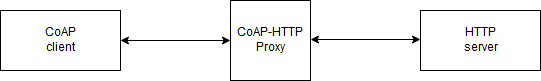
\includegraphics[width=\linewidth]{coap-img1.png}
		\caption{Example of CoAP proxy.}
		\label{fig:coap1}
	\end{figure}

	A proxy in CoAP is an endpoint that acts as broker between client and server, basically it receives a request, translates it and forwards the request to the origin server.
	
	When dealing with proxies we can identify two classes:
	\begin{itemize}
		\item CoAP to CoAP Proxies
		\item Cross Protocol Proxies
	\end{itemize}
	
	A proxy can have a cache or not, in the former case if the server does not have a fresh response for the request it will need to refresh its cache, then it will translate the request and forward a new crafted request to the origin server; in the latter case the proxy receives the request, translate it and forwards the new request to the origin server.
	
	A proxy with a cache must not extend the \texttt{Max-Age} Option of a response while it forwards the response to the client; the proxy could adjust the \texttt{Max-Age} in this way:
	\begin{equation}
		proxyMaxAge=originalMaxAge-cacheAge
	\end{equation}
	
	When a proxy does not recognize a certain Option, it must send back a 4.02 response.\newline
	A proxy must forward all Safe-To-Forward options, but it must send back a 5.02 response if an unsafe option is not recognized.\newline
	In case of timeout the proxy must return a 5.04 response, if a response cannot be processed by the proxy a 5.02 must be returned.\newline
	
	A proxy receives a request and it need to know which parameters it must use in order to create the new request and forward it to the server.\newline
	This procedure is fully defined to a forward proxy, but there is no specification of a reverse proxy.\newline
	
	A forward proxy receives a request with the Proxy-Uri or the Proxy-Scheme Option, from one of these options it will determine the component of the request URI and will split them in:
	\begin{itemize}
		\item Uri-Host
		\item Uri-Port
		\item Uri-Path
		\item Uri-Query
	\end{itemize}

	Proxy-Uri and Proxy-Scheme are not forwarded in the new request.\newline
	A reverse proxy receives requests without the Proxy-Uri or Proxy-Scheme; it needs to determine the destination of a request from the request itself and from its configuration.\newline
	It could discover new resources via Resource Discovery and it can offer them as they were its own.\newline
	
	When a client uses a proxy to make a request with TLS, the request towards the proxy should be done with TLS; there is no guarantee that the proxy will use TLS, so be careful.\newline
	
	\subsection{CoAP-HTTP Proxying}
	As mentioned before, it is possible to implement a proxy between CoAP and HTTP.\newline
	Figure \ref{fig:coap2} illustrates where the proxy is placed in the communication between the client and the server.
	
	\begin{figure}
		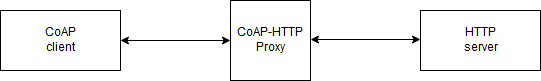
\includegraphics[width=\linewidth]{coap-img1.png}
		\caption{Example of CoAP to HTTP proxy.}
		\label{fig:coap2}
	\end{figure}
	
	When a CoAP endpoint sends a request including the Proxy-Uri or Proxy-Scheme option with a HTTP or HTTPS URI, the receiving proxy will translate the CoAP message into an HTTP or HTTPS request and perform the operation specified in the original request.\newline
	If the proxy is not capable of handling the submitted request, a 5.05 response is returned to the client.\newline

	Since the CoAP methods are a subset of the HTTP methods, so each method can be mapped to its corresponding one.

	
	\subsection{HTTP-CoAP Proxying}
	It is also possible to perform the inverse proxying operation from HTTP to CoAP.\newline
	However there are some restrictions, because some methods of HTTP are not supported by CoAP.
	
	In this case the mapping between the two protocols is not always possible, HTTP methods like
	OPTION and TRACE are not supported, for this reason the proxy must return a 501 error.\newline
	The supported methods are:
	\begin{itemize}
		\item GET
		\item PUT
		\item POST
		\item DELETE
		\item HEAD
	\end{itemize}
	
	\section{CoAP URI}
	CoAP uses \emph{coap} and \emph{coaps} URI schemes as a means of locating the resource.
	The first is used for unencrypted communication; the second is used for encrypted communication.
	
	Resources are organized in a hierarchic way and they are governed by an origin server that listens for request.
	
	A coap-URI is defined as follows:\\
	\texttt{Coap-URI=”coap:” “//” host [“:” port] path-abempty [“?” query]}\\
	If the host is an ip-literal or an IPv4, it can be reached at that IP address, on the other hand if it is a registered name, it is an indirect identifier and it must be resolved via DNS.\newline
	If the host is empty, then the URI is invalid.\newline
	The default port is 5683.\newline
	The path identifies a resource and it is a string separated by slash.\newline
	The query is used to provide parameter to the resource, it is a sequence of argument separated by an ampersand (\&).
	
	A coaps-URI is defined as follows:\\
	\texttt{coaps-URI = "coaps:" "//" host [ ":" port ] path-abempty [ "?" query ]}\\
	The differences are: the s after \texttt{coap}, the default port which is 5684 and the UDP datagrams must be secured with DTLS.
	It is important to highlight that two resources with the same name, but made available, one via \texttt{coap}, and the other via \texttt{coaps}, are unrelated.
	
	The most of URI handling is delegated to the client; in fact it parses the URI and splits it into:\newline
	\begin{itemize}
		\item Host
		\item Port
		\item Path
		\item Query components
	\end{itemize}
	
	\section{Multicast CoAP}
	CoAP supports requests to a multicast group IP; if a server wants to make its resources discoverable, it needs to join one of the following multicast address:
	\begin{itemize}
		\item IPv4: 224.0.1.187
		\item IPv6 ff0x:fd
		\item Other multicast addresses
	\end{itemize}

	An endpoint must be prepared to receive multicast requests even from different addresses, if an endpoint is not interested in sharing its resources it can simply ignore the requests.\newline
	
	At the messaging layer, a multicast request is transported in a CoAP NON message with a multicast IP address.\newline
	In order to avoid an explosion of error responses, an endpoint must not return a RST message to a NON message.\newline
	Take in mind that multicast requests are not supported by DTLS but only by UDP.\newline
	
	When an endpoint receives a multicast request, it could ignore the request whenever it does not have anything useful to send back; on the other hand if it chooses to respond, it will respond but not immediately, only after a certain amount of time, the length of the period is called \textbf{leisure}.\newline
	The leisure is defined by the application or by this simple equation:
	\begin{equation}Leisure=S\cdot\frac{G}{R}\end{equation}
	Where $G$ is the estimated group size, $R$ is the transfer rate and $S$ the response size, it expresses a lower bound.\newline
	
	The server chooses a random point of time within the leisure to send a unicast response; 
	each time a further response needs to be sent, a new leisure period must be defined.\newline
	
	In order to match a response to a multicast request, only the token must match.\newline
	
	\section{Discovery}
	A client can find a server in three different ways:
	\begin{itemize}
		\item It knows the URI
		\item It learns the URI
		\item Or it finds out via multicast request
	\end{itemize}

	A server that supports resource discovery must use the default port 5683.\newline
	
	In a M2M environment where there is no human intervention it is very important to have a way to discover resources.\newline
	A server that support resource discovery should support the CoRE (Constrained Restful Environment) link format of discoverable-resource (RFC 6690) when manual configuration is missing.\newline
	
	\section{Securing CoAP}
	CoAP can operate in one of the security modes listed in table \ref{tab:table10}.
	
		\begin{table}[h!]
		\begin{center}
			\begin{tabularx}{\textwidth}{|l|X|}
				\hline
				NoSec & In this mode there is no security because DTLS is disabled.
				Basically, messages are sent over the normal UDP channel and the coap scheme is used.\\\hline
				PreSharedKey & DTLS is enabled and the device has a list of pre-shared keys that it uses to communicate with the other nodes in the network.
				It is possible to have a one key for each node in the network but it may be not possible for memory constraint.
				It uses the coaps scheme.
				When an endpoint starts a communication with another endpoint an appropriate key is selected.
				The cipher suite must implement \texttt{TLS\_PSK\_WITH\_AES\_128\_CCM\_8}.\\\hline
				RawPublicKey & DTLS is enabled and the device has an asymmetric key but no certificate.
				It uses the coaps scheme.
				The symmetric key is generated and installed by the manufacturer of the device.
				A device may have multiple public keys.
				The cipher suite must implement \texttt{TLS\_ECDHE\_ECDSA\_WITH\_AES\_128\_CCM\_8}.\\\hline
				Certificate & DTLS is enabled and the device has an asymmetric key and a signed certificate.
				The device has a list of root trust that it uses to validate the certificate.
				It uses the coaps scheme.
				The certificate needs to be verified when a new connection is created, if the CoAP node is capable of computing an absolute time, then the node should check the validity of the certificate.
				The cipher suite must implement \texttt{TLS\_ECDHE\_ECDSA\_WITH\_AES\_128\_CCM\_8}.\\\hline
				
				
			\end{tabularx}
			\caption{Security options available in CoAP.}
			\label{tab:table10}
		\end{center}
	\end{table}
	
	It is important to highlight that we are dealing with constrained devices; in some cases, it could be possible that the available resources are not able to support a secure communication, or the support of a certain cipher suite is only partial.\newline
	Also, take in mind that DTLS adds a little overhead and it could slow down the communication or create congestion in the network.\newline
	
	Of course, the use of DTLS is strongly recommended, but in some case it could be simply impossible to use, thus the network is secure, only if an attacker is not capable of sending and receiving messages.\newline
	Also, take in mind that DTLS is not supported for multicast CoAP messages.\newline
	
	While using DTLS, all CoAP messages must be sent as DTLS “application data”, in order to match an ACK or RST message to a CON the DTLS session must be the same, the rules apply even for the epoch.\newline
	The same for matching a RST message to a NON messages.\newline
	
	During the retransmission of a CON message, a new DTLS sequence number is used at each attempt, but the Message ID does not change.\newline
	Retransmission must not be performed across epochs.\newline
	
	In order to match a request to a response there is a new rule: the DTLS session must match and even the epoch must match, thus a DTLS request must always associated to a DTLS response, if the response is not secured it must be rejected.
	
	\section{Security perspective}
	Every protocol has some flaws in its design and in its implementations; by exploiting these flaws is it possible to perform attack, from a simple denial of service to a remote code execution.\newline
	A DoS may be possible by exploiting a flaws in the protocol, for a remote code execution a big flaw in the implementation must be present, of course an error in the design could accentuate an implementation flaw.\newline
	
	In this section we will not talk about specific attack but only list down some hypothesis, we will talk about real attack in another chapter.\newline
	
	One source of flaws for CoAP could be the parser that analyze the messages; a parser is a program that recognize a grammar, if the grammar is complex then its parser will not be less complex, it is trivial to understand that it is likely that a flaw may hide inside the parser, this could lead to DoS or remote code execution if a buffer overflow happens.\newline
	
	Talking about URI processing, CoAP moved the most of it on the client side to avoid vulnerabilities server side, in this case, the vulnerabilities could be in the client side, the IETF suggest to take special care while implementing the URI processing.\newline
	
	The fact that most constrained device will execute, for performance reasons, the protocol implemented in C it is likely that a buffer overflow could happen if the memory is not handled properly. \newline
	
	A proxy is, from the security point of view, a man in the middle; if a proxy endpoint is compromised, even using DTLS is useless.\newline
	If a proxy also performs caching tasks, an attacker could carry out a DoS by caching forever useless messages or old real messages.\newline
	
	When a server replies to a request, the response may be larger than the request packet.\newline
	We could exploit a CoAP server in order to generate a huge amount of network traffic with the aid of IP spoofing; this is a particular case of DoS known as amplification attack.\newline
	This could be particularly interesting because we are dealing with constrained devices, so suppose that somehow, we have taken control of a node, but that it is not powerful enough to perform a DoS alone, we could exploit a CoAP server, which we assume is quite more powerful of a single node, to generate a huge network traffic.\newline
	On the other hand, a constrained network could only be able to generate a small amount of traffic due to the fact that is constrained by design.\newline
	It is possible to avoid this particular attack if the nodes are authenticated.\newline
	
	Another source of attack could be the use of multicast IP, but as we have seen the protocol specify a particular procedure in order to avoid DoS attack on this front.\newline
	In order to avoid attacks via multicast IP a server should not accept a request that could not be authenticated.
	
	Due to the nature of UDP an endpoint can read messages carried by the network if the configuration is NoSec or PreSharedKey.\newline
	It is possible to spoof a RST message in response to a CON or NON message.
	An attacker could send an ACK in response to a CON in order to prevent the retransmission of a message and thus blocking the endpoint.\newline
	
	Also take in mind that the fact we are dealing with constrained device is quite important, another possible attack could be a DoS that tries to exhaust the energy of a constrained device in order to shut it down, this is possible by forcing an endpoint to retransmit a message or by sending multicast messages.\newline
	
	A constrained device may not have enough entropy in order to provide secure pseudo-random number generator, this could lead to trivial and predictable token.\newline
	
	Due to the limited resources, a constrained device may be susceptible to timing attack, in particular while dealing with cryptographic primitive.\newline
	
	Another possible threat is given by the environment where the constrained device is deployed, if the environment is not properly secured an attacker could simply tamper the device or, if his target is creating a DoS, by smashing the device with a hammer.\newline
	So it is important to place constrained devices in a controlled environment in order to avoid attacks that are not completely related with the digital world.\newline
	
	\section{Differences and short comparison with MQTT}
	Both CoAP and MQTT are good for constrained environment, but they have different targets and features, CoAP uses UDP as underlying transport layer, while MQTT uses TCP that supports an advanced reliability model compared to CoAP.\newline
	
	CoAP is easily mapped to HTTP because it was designed with this feature in mind.\newline
	
	MQTT is most suitable for event-based communication while CoAP is a better choice for continuous monitoring scenario.\newline
	CoAP also offers faster communication compared to MQTT and it is more indicated for M2M communication, on the other hand, CoAP is UDP based and unreliable by design; while MQTT thanks to TCP is reliable, but slower.\newline
	
	MQTT is more common compared to CoAP; that is because MQTT was adopted, at least initially, by the big cloud player.\newline
	Another factor to take in mind is the specification's release date: MQTT was released in 1999 while CoAP in 2014; this is why CoAP is, at the moment, less widespread.\newline
	
	\section{CoAP implementation}
	At this link: \url{http://coap.technology/impls.html} are listed some CoAP implementations.\newline
	All the most important programming languages are supported.\newline
	For constrained devices the libraries are written, most of the time, in low level languages like C, note that some library are specifically written for a certain class of constrained device, for example tinydtls is a library that implements DTLS for class 1 devices.\newline
	
	There is also a library for less constrained devices where it is possible to run a JavaScript interpreter.\newline
	
	From the server side point of view, there are implementations for every important language like C, Java, C\# and JavaScript.\newline
	
	There are also implementation for mobile devices and closed source implementation; one in particular is developed by ARM.\newline
	
	At the moment there is no known real world application that uses CoAP heavily, but the amount of scientific paper about this protocol may lead to an adoption from the company.
	\newline
	
	I also find out that there is an implementation of a HTTP/CoAP proxy.\cite{rossini2012design}.